\documentclass[tikz,border=10pt]{standalone}
\usepackage{pgfplots} % Load the pgfplots package
\pgfplotsset{compat=1.18} % Set compatibility to a recent version

\begin{document}
	
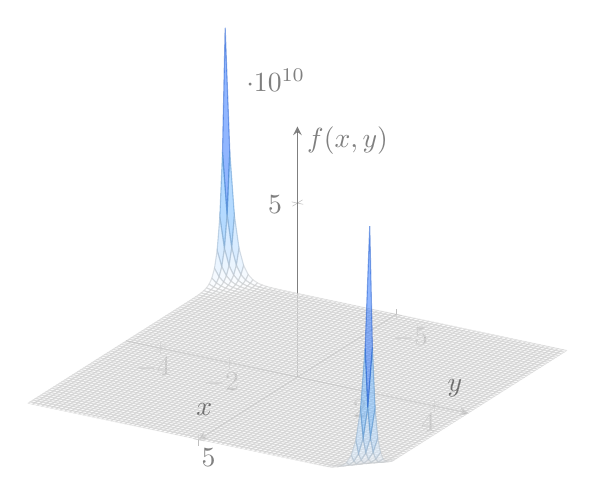
\begin{tikzpicture}
\begin{axis}[
%	title={$f(x, y) = y - x^2$}, % Title of the plot
	xlabel={$x$}, % Label for the x-axis
	ylabel={$y$}, % Label for the y-axis
	zlabel={$f(x,y)$}, % Label for the z-axis
	grid=major, % Display major grid lines
	colormap/cool,
	opacity=0.5,
	axis lines = middle,
	view={120}{30},
	]
	\addplot3[
		surf,            % Draw a surface plot
	%	shader=interp,   % Use interpolated shading for a smooth look
		domain=-5:5,     % x-range
		domain y=-5:5,   % y-range
		samples=75,      % Number of sample points for a smoother surface
		]
	{x*x*y + exp(x*y)}; % The function to plot
\end{axis}
\end{tikzpicture}
	
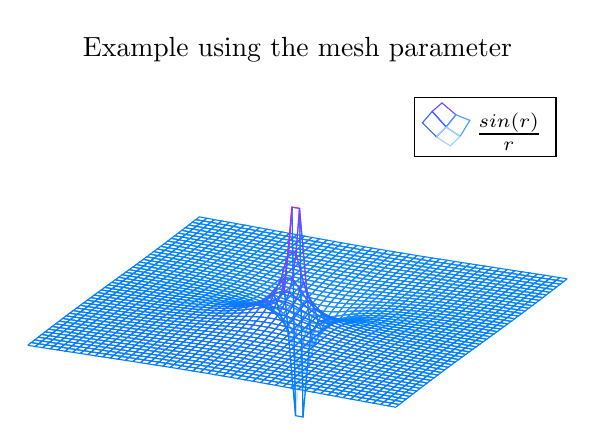
\begin{tikzpicture}
	\begin{axis}[
		title=Example using the mesh parameter,
		hide axis,
		colormap/cool,
		]
		\addplot3[
		mesh,
		samples=50,
		domain=-10:10,
		]
		{-y / (x*x+y*y)};
		\addlegendentry{\(\frac{sin(r)}{r}\)}
	\end{axis}
\end{tikzpicture}
	
\end{document}



%\documentclass[tikz,border=10pt]{standalone}
%\usepackage{amsmath}
%\usepackage{pgfplots}
%
%\begin{document}
%	
%\begin{tikzpicture}
%\begin{axis}[
%	axis lines = middle,
%	xlabel = $x$, ylabel = $y$, zlabel = {$f(x, y)$},
%%	title = {Surface of $f(x, y) = x^2 y + e^{xy}$},
%%	width=10cm, height=10cm,
%%	domain=-5:5, y domain=-5:5,  samples=30,
%	colormap/cool,
%	grid = major, opacity=0.5,
%	view={125}{30}  % Azimuth = 120, Elevation = 30
%	]
%	\addplot3[surf, domain=-2:2, y domain=-2:2, samples=30] {y-x*x};
%\end{axis}
%\end{tikzpicture}
%%\begin{tikzpicture}
%%	\begin{axis}[
%%%		axis lines = middle,
%%%		xlabel = {$x$}, ylabel = {$y$}, zlabel = {$f(x, y)$},
%%		domain=-15:15, y domain=-15:15,  samples=30,    
%%		xmin=-15, xmax=15,   % Set the length of the x-axis
%%		ymin=-15, ymax=15,   % Set the length of the y-axis
%%%		zmin=-15, zmax=15,   % Set the length of the z-axis
%%		colormap/cool,
%%		grid = major, opacity=0.5,
%%		view={120}{60}, % Set the view angle (azimuth and elevation)
%%		]
%%		\addplot3[
%%		surf,
%%		]
%%		{y-x*x};
%%	\end{axis}
%%\end{tikzpicture}
%\end{document}
